\documentclass[margin=5mm]{standalone}
\usepackage[dvipsnames]{xcolor}
\usepackage{pgfplots}
\usepackage{tikz}
\usepackage[tikz]{ocgx2}

\pgfplotsset{compat=1.18}
\begin{document}

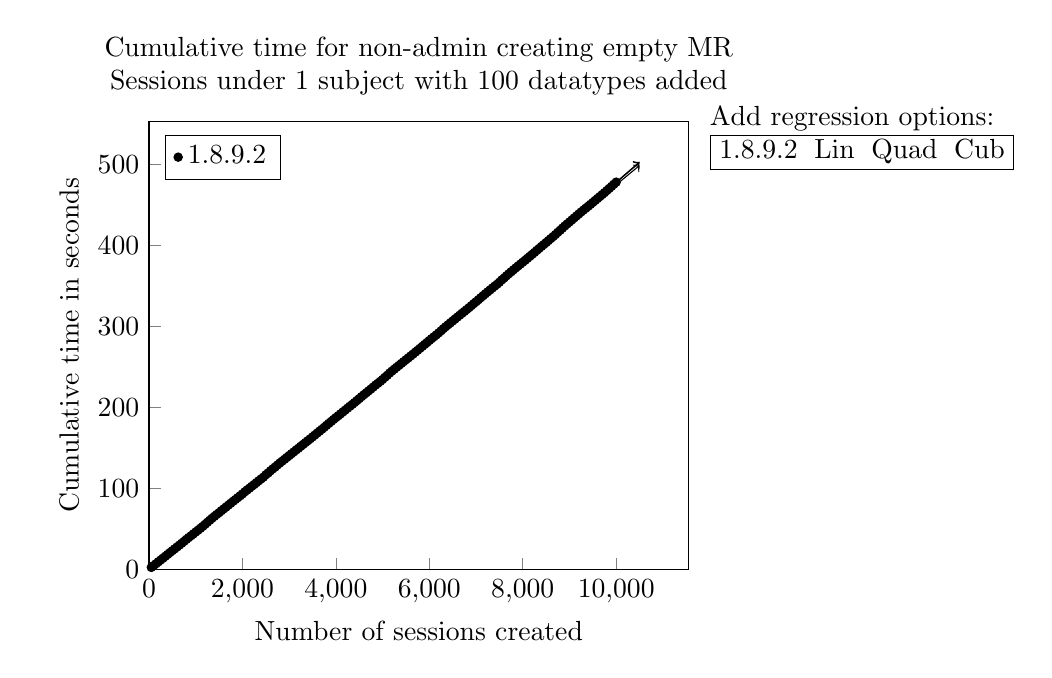
\begin{tikzpicture}
    \begin{axis}[
        align = center,
        legend pos = north west,
        legend cell align = left,
        xlabel = Number of sessions created,
        ylabel = Cumulative time in seconds,
        xtick pos = left,
        ytick pos = left,
        scaled ticks = false,
        xmin = 0,
        ymin = 0,
        title = {Cumulative time for non-admin creating empty MR Sessions under 1 subject with 100 datatypes added},
        title style = {text width = 0.8\textwidth},
        legend entries={\switchocg{1.8.9.2}{1.8.9.2}}]
        \begin{scope}[ocg = {ref = 1.8.9.2-Lin, status = invisible}]
            \plot[domain=0:10500,->,forget plot] (\x,{-2.513124924623161060566189917153678834438323974609375 + 0.047735755208880230326951021879722247831523418426513671875*(\x)^1});
        \end{scope}
        \begin{scope}[ocg = {ref = 1.8.9.2-Quad, status = invisible}]
            \plot[domain=0:10500,->,forget plot] (\x,{0.318835791837903503864737331241485662758350372314453125 + 0.046053402308012268695502910986760980449616909027099609375*(\x)^1 + 0.000000167398298593827558817368384054546925909789933939464390277862548828125*(\x)^2});
        \end{scope}
        \begin{scope}[ocg = {ref = 1.8.9.2-Cub, status = invisible}]
            \plot[domain=0:10500,->,forget plot] (\x,{-0.19737235966031330125503018280141986906528472900390625 + 0.046662192037867235294701373504722141660749912261962890625*(\x)^1 + 0.000000016335092770822064320160584504314227327625985708436928689479827880859375*(\x)^2 + 0.00000000001002077650567200536770798933218303461596676573464037574012763798236846923828125*(\x)^3});
        \end{scope}
        \begin{scope}[ocg = {ref = 1.8.9.2, status = visible}]
            \addplot[
                only marks,
                color = black,
                mark = *,
                mark size = 1.5 pt
            ]coordinates {(50,2.473)(100,4.711)(150,6.967)(200,9.35)(250,11.575)(300,13.9)(350,16.236)(400,18.515)(450,20.853)(500,23.112)(550,25.363)(600,27.662)(650,29.916)(700,32.254)(750,34.609)(800,37.031)(850,39.306)(900,41.547)(950,43.839)(1000,46.155)(1050,48.419)(1100,50.739)(1150,53.051)(1200,55.571)(1250,58.168)(1300,60.657)(1350,63.122)(1400,65.496)(1450,67.808)(1500,70.043)(1550,72.48)(1600,74.712)(1650,77.016)(1700,79.369)(1750,81.661)(1800,84.052)(1850,86.291)(1900,88.5)(1950,90.851)(2000,93.171)(2050,95.718)(2100,97.996)(2150,100.25)(2200,102.558)(2250,104.775)(2300,107.098)(2350,109.452)(2400,111.7)(2450,113.911)(2500,116.704)(2550,119.083)(2600,121.714)(2650,124.087)(2700,126.387)(2750,128.909)(2800,131.313)(2850,133.635)(2900,135.875)(2950,138.199)(3000,140.51)(3050,142.851)(3100,145.107)(3150,147.452)(3200,149.655)(3250,152.011)(3300,154.341)(3350,156.637)(3400,158.888)(3450,161.22)(3500,163.574)(3550,165.885)(3600,168.335)(3650,170.683)(3700,172.951)(3750,175.349)(3800,177.845)(3850,180.227)(3900,182.711)(3950,185.059)(4000,187.399)(4050,189.663)(4100,192.01)(4150,194.375)(4200,196.684)(4250,199.063)(4300,201.4)(4350,203.672)(4400,206.028)(4450,208.413)(4500,210.852)(4550,213.328)(4600,215.661)(4650,218.015)(4700,220.355)(4750,222.677)(4800,225.111)(4850,227.572)(4900,229.797)(4950,232.119)(5000,234.485)(5050,237.165)(5100,239.655)(5150,242.387)(5200,244.821)(5250,247.188)(5300,249.518)(5350,251.825)(5400,254.23)(5450,256.499)(5500,258.835)(5550,261.127)(5600,263.418)(5650,265.747)(5700,268.169)(5750,270.455)(5800,272.893)(5850,275.327)(5900,277.715)(5950,280.054)(6000,282.547)(6050,284.912)(6100,287.241)(6150,289.563)(6200,291.966)(6250,294.476)(6300,297.166)(6350,299.585)(6400,301.952)(6450,304.359)(6500,306.681)(6550,309.087)(6600,311.495)(6650,313.791)(6700,316.168)(6750,318.465)(6800,320.803)(6850,323.152)(6900,325.592)(6950,328.044)(7000,330.455)(7050,332.894)(7100,335.38)(7150,337.816)(7200,340.293)(7250,342.688)(7300,345.018)(7350,347.435)(7400,349.746)(7450,351.957)(7500,354.515)(7550,357.334)(7600,359.715)(7650,362.443)(7700,364.907)(7750,367.383)(7800,369.785)(7850,372.184)(7900,374.575)(7950,376.92)(8000,379.267)(8050,381.59)(8100,384.052)(8150,386.409)(8200,388.885)(8250,391.267)(8300,393.775)(8350,396.233)(8400,398.719)(8450,401.061)(8500,403.503)(8550,405.967)(8600,408.447)(8650,410.87)(8700,413.363)(8750,416.167)(8800,418.693)(8850,421.333)(8900,423.975)(8950,426.508)(9000,428.92)(9050,431.372)(9100,433.92)(9150,436.365)(9200,438.803)(9250,441.329)(9300,443.641)(9350,445.975)(9400,448.315)(9450,450.638)(9500,453.031)(9550,455.523)(9600,457.907)(9650,460.308)(9700,462.728)(9750,465.131)(9800,467.712)(9850,470.297)(9900,472.777)(9950,475.52)(10000,478.112)};
        \end{scope}
    \end{axis}
    \begin{scope}
        \addtolength{\tabcolsep}{-0.3em}
        \node [below right, shape=rectangle, align=left](regressiontable) at (7,6) {
            Add regression options: \\
            \begin{tabular}{|llll|}
                \hline
                1.8.9.2 & \switchocg{1.8.9.2-Lin}{Lin} & \switchocg{1.8.9.2-Quad}{Quad} & \switchocg{1.8.9.2-Cub}{Cub} \\
                \hline
            \end{tabular}
        };
    \end{scope}
\end{tikzpicture}

\end{document}